\section{ГЕНЕРАЦИЯ СЛУЧАЙНЫХ ГРАФОВ}
Для многих задач требуется генерация 
случайного графа. Будут рассмотрены 
разные модели генерации случайного графа \cite{rnd}. Каждая 
модель представлена отдельным модулем.
\subsection{Модель Эрдеша-Ренье}
Рассмотрим простейшую модель генерации случайного графа. 
Даны $n \in \mathbb{N}, p \in (0,1)$. Создается 
полный граф с $n$ вершинами, каждое
ребро берется с вероятностью  $p$.

\begin{figure}[H] 
\begin{lstlisting}[language=Python] 
    def complete_graph_edges(k):
        edges = []
        for a in range(1, k+1):
            for b in range(a+1, k+1):
                edges.append((a, b))
                edges.append((b, a))
        return edges
\end{lstlisting}  
\caption{Генерация списка ребер полного графа с
$k$ вершинами}
\label{erd_1}
\end{figure}
\begin{figure}[H] 
\begin{lstlisting}[language=Python] 
    def erdos_renyi_random_graph(n, p):
        edges = [e for e in ErdosRenyiGraph.complete_graph_edges(
            n) if random() < p]
        g = Graph()
        g.add_edges(edges)
        g.add_vertecies(range(1, n+1))
        return g
\end{lstlisting}  
\caption{Генерация случайного графа по модели Эрдеша-Ренье }
\label{erd_2}
\end{figure} 
На рисунках \ref{erd_1},\ref{erd_2}
приведен код для генерация случайного графа.
\begin{figure}[H] 
    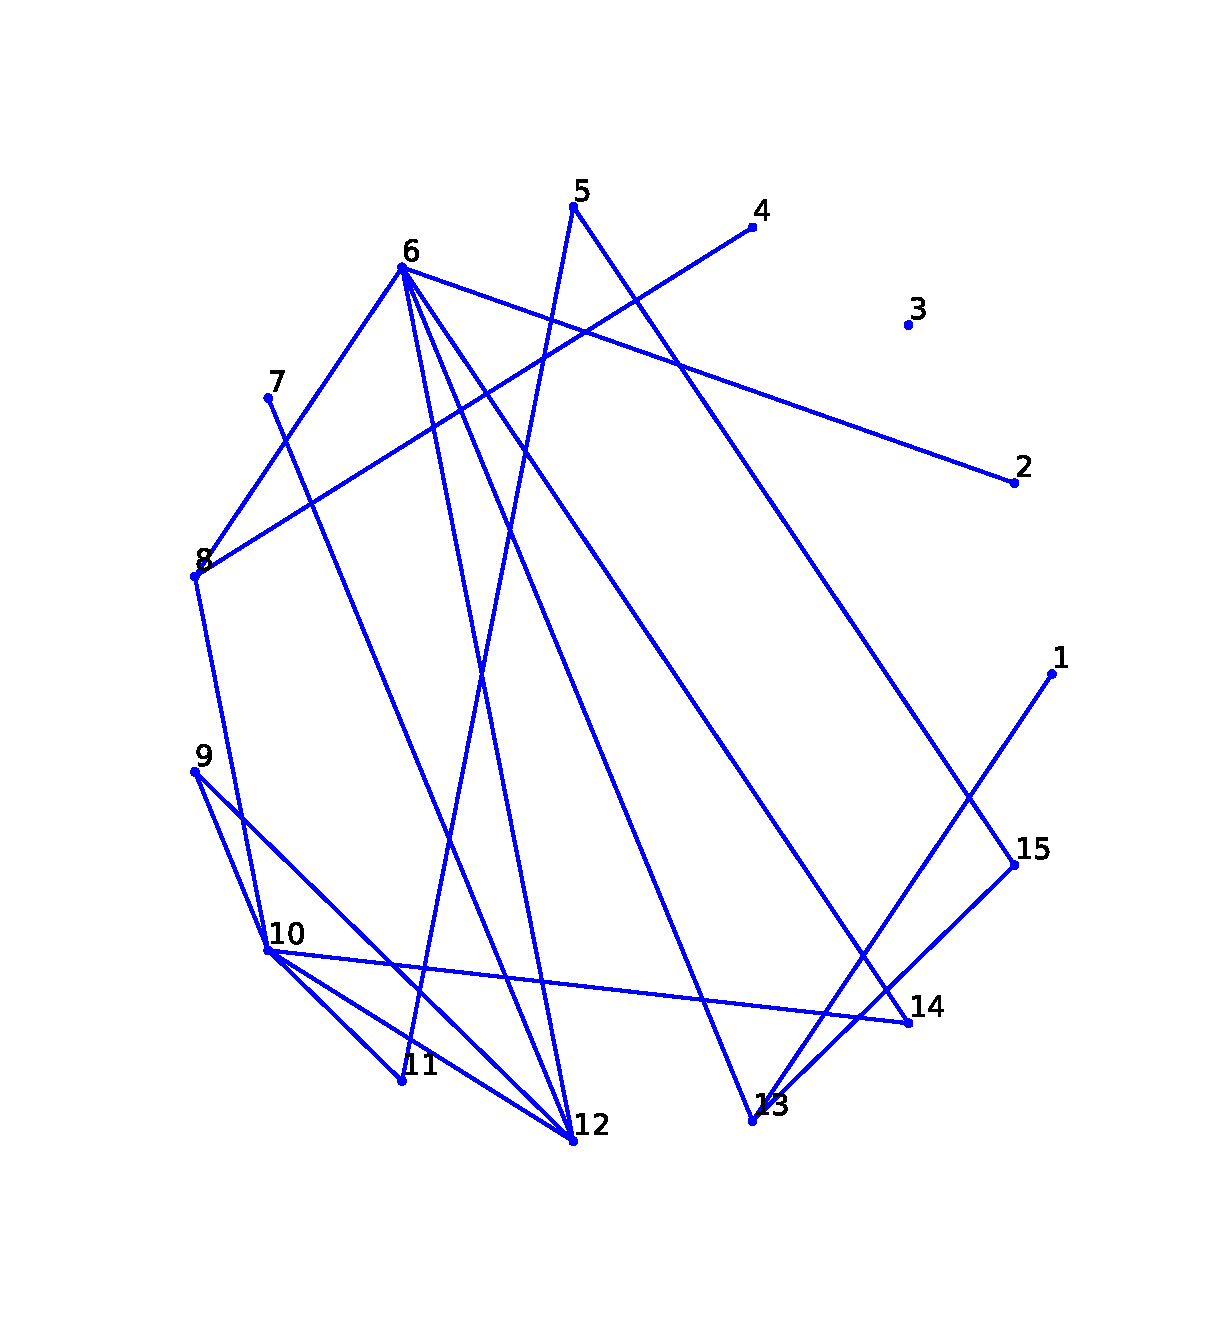
\includegraphics[scale=0.5]{erd1.pdf} 
    \caption{Случайный граф созданный с помощью модели Эрдеша-Ренье с
    параметрами $n = 15, p = 0.1$}
    \label{erd_3}
\end{figure} 
\begin{figure}[H] 
    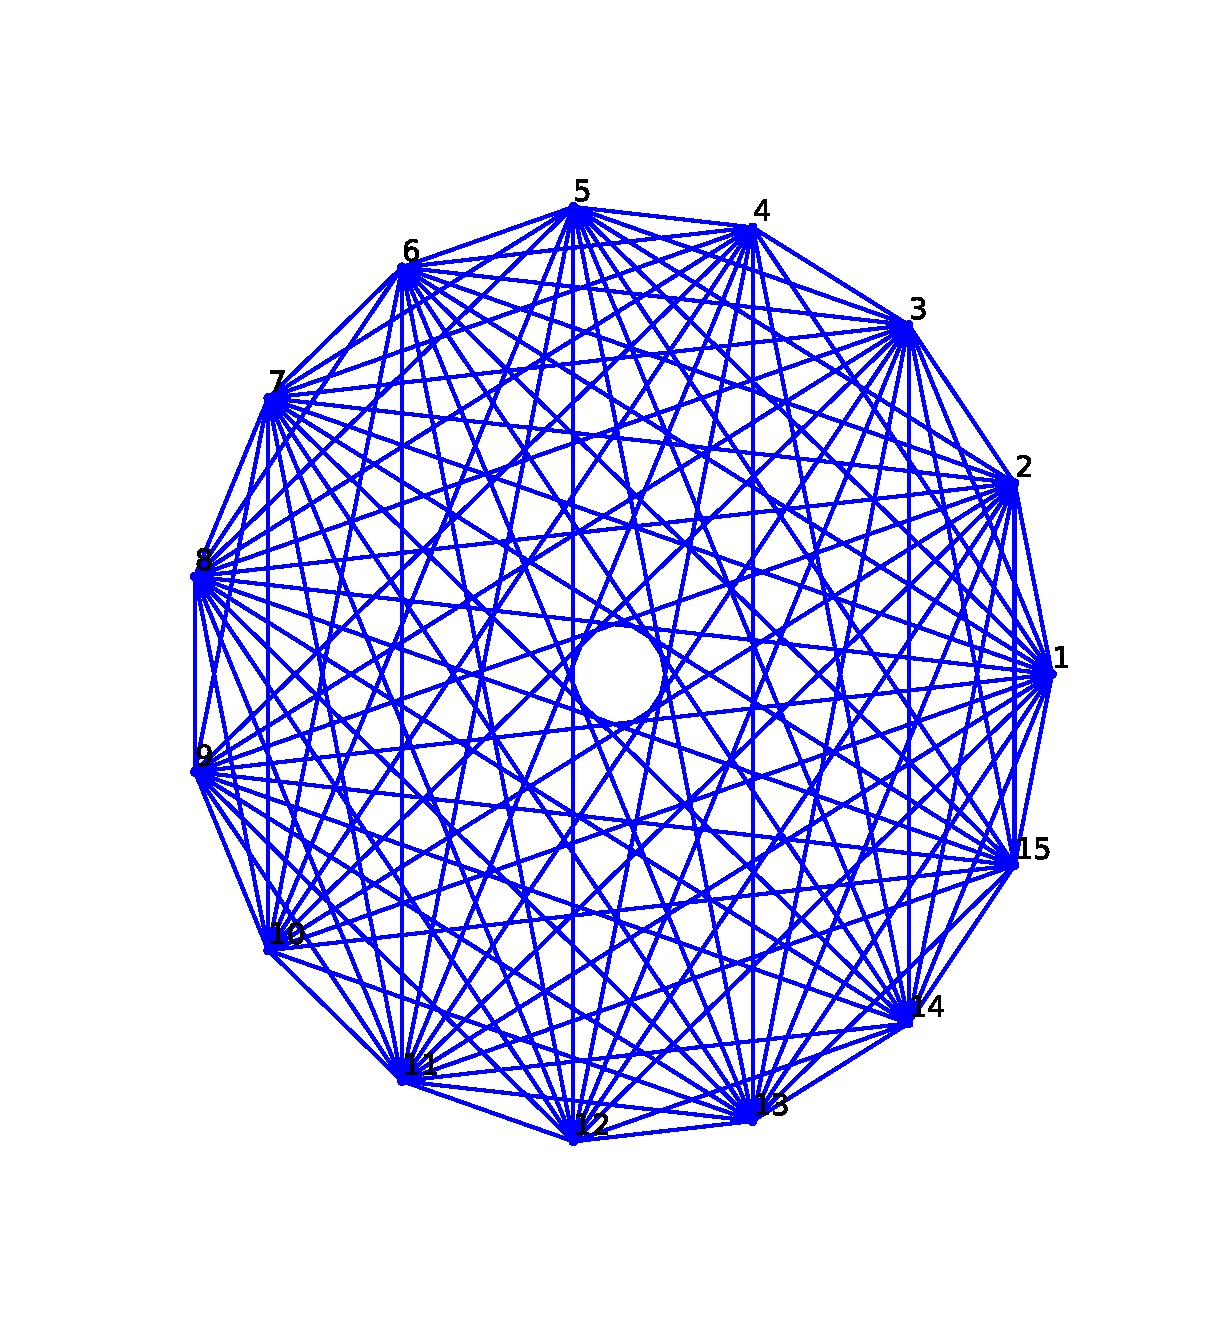
\includegraphics[scale=0.5]{erd2.pdf}
    \caption{Случайный граф созданный с помощью модели Эрдеша-Ренье с
    параметрами $n = 15, p = 0.7$}
    \label{erd_4}
\end{figure} 
На рисунках \ref{erd_3}, \ref{erd_4}
приведены примеры графов, созданных с помощью
данной модели. 

Графы созданные с помощью модели Эрдеша-Ренье плохо
описывают реальные сетевые структуры такие, как 
социальные сети. 
\subsection{Модель Барабаши-Альберт}
Пусть дан граф с $n$ вершинами и  $m \le n \in \mathbb{N}$.
Будем добавлять вершины пошагово, 
каждая добавленная вершина должна 
иметь $m$ ребер. 
 \begin{equation}
     P_{in} = \frac{\deg{i}}{ \sum_{j} \deg{j}}
     \label{ba}
\end{equation} 
Формула \ref{ba} обозначает вероятность добавления ребра
$\{i,n\}$
\begin{figure}[H] 
\begin{lstlisting}[language=Python] 
    def add_vertex(self, vertex):
        if vertex not in self.graph.verticies():
            total_deg = sum(self.graph.deg(v) for v in self.graph.verticies())
            p = [self.graph.deg(v) / total_deg for v in self.graph.verticies()]
            end = choice(list(self.graph.verticies()),
                         p=p, size=self.m, replace=False)
            for v1 in end:
                self.graph.add_edge(vertex, v1)
\end{lstlisting}  
    \caption{Реализация добавления вершины согласно модели Барабаши-Альберт}
    \label{ba_1}
\end{figure} 
На рисунке \ref{ba_1} приведен код, который реализует 
добавление новой вершины в граф, согласно данной модели.
\begin{figure}[H] 
    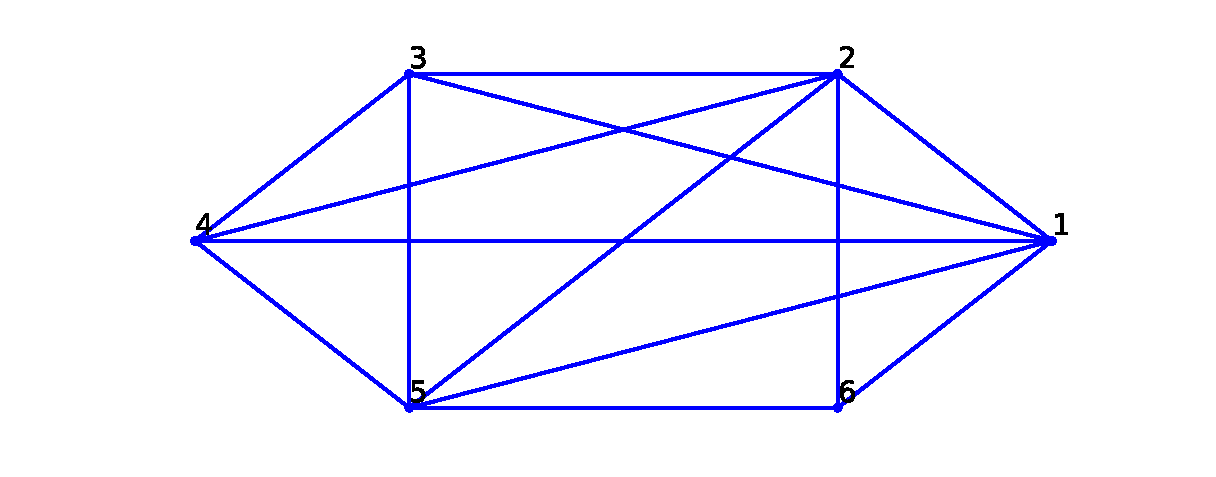
\includegraphics[scale=0.4]{ba1.pdf} 
    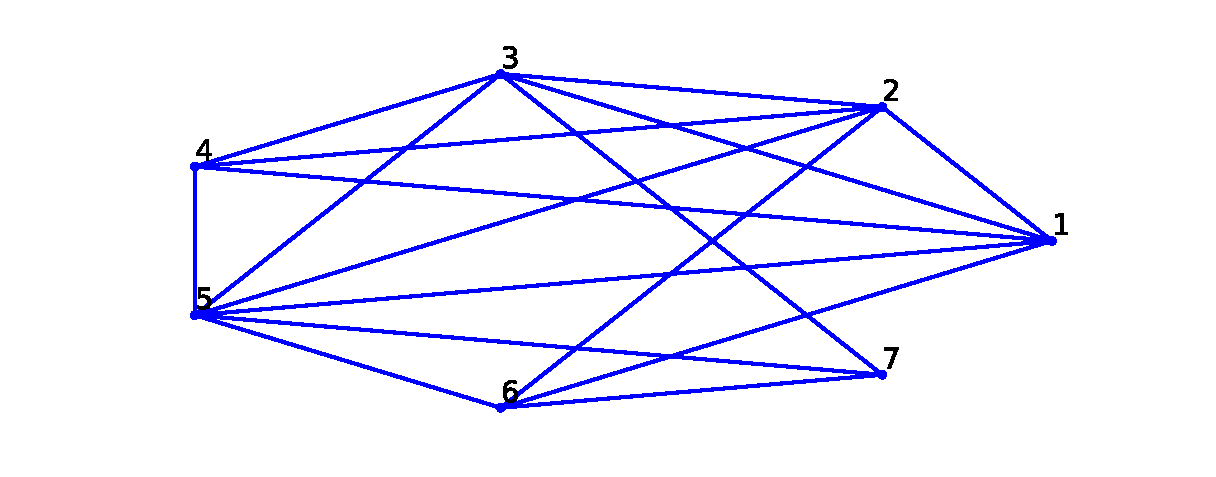
\includegraphics[scale=0.4]{ba2.pdf} 
    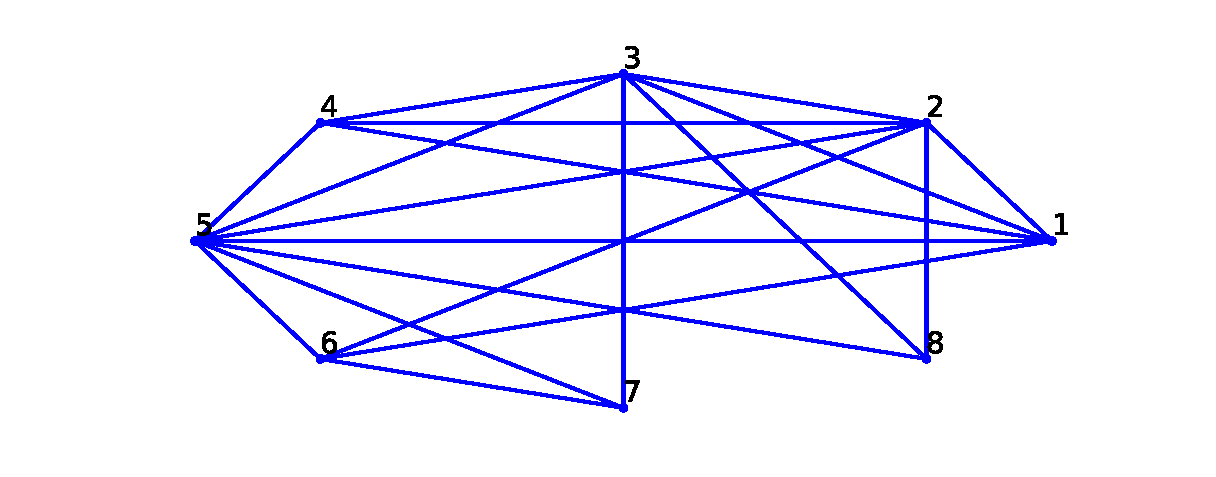
\includegraphics[scale=0.4]{ba3.pdf} 
    \caption{Визуализация построения 
    случайного графа с помощью модели Барабаши-Альберт с параметрами
$n=5,m=3$}
\label{ba_4}
\end{figure} 
На рисунке \ref{ba_4} приведны три шага итерации построения
случайного графа, согласно модели Барабаши-Альберт.
\subsection{Модель Боллобаша-Риордана}
Пусть дан граф с одной вершиной и петлей. 
Добавляем пошагово вершины. Пусть граф с $n-1$ 
вершиной построен, тогда 
$P_{in} = \frac{\deg{i}}{2n - 1}$, $P_{nn} = \frac{1}{2n - 1}$
\begin{figure}[H] 
\begin{lstlisting}[language=Python] 
    def __init__(self, n):
        g = Graph()
        g.add_edge(1, 1)
        for v in range(2, n+1):
            p = [g.deg(vertex) / (2*n - 1) for vertex in g.verticies()]
            p.append(1 / (2*n - 1))
            g.add_vertex(v)
            end = choices(list(g.verticies()), weights=p, k=1)
            g.add_edge(v, end[0])
        self.graph = g
\end{lstlisting}  
    \caption{Построение графа с $n$ вершинами, согласно модели 
    Боллобаша-Риодана.}
    \label{br_1}
\end{figure} 
На рисунке \ref{br_1} приведен код для генерации случайного графа
c помощью модели Боллобаша-Риодана.
\begin{figure}[H] 
    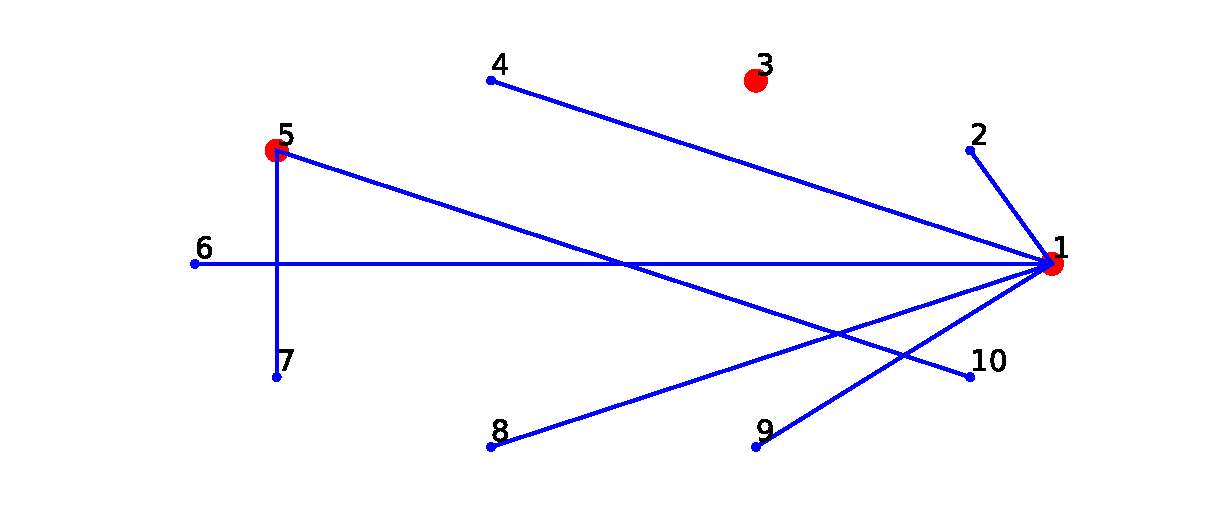
\includegraphics{br.pdf} 
    \caption{Граф с 10 вершинами, построенный согласно модели
    Боллобаша-Риодана}
    \label{br_2}
\end{figure} 
На рисунке \ref{br_2} изображен граф построенный согласно данной модели.
\subsection{Модель Боллобаша-Риодана для создания ориентированного графа}
Рассмотрим следущую модель генерации случайного ориентированного графа \cite{bolor}. Пусть даны неотрицательные вещественные числа 
$\alpha,\beta,\gamma,\delta_{\text{in}},\delta_{\text{out}}$, где
$\alpha + \beta + \gamma = 1$ и ориентированный граф  $G(1)$.
Будет создаваться последовательность $G(1),G(2),\dots, G(t),G(t+1) \dots G(n)$, где следущий граф строится по предыдущему.
Пусть вершина  $v \in V(t)$ выбирается согласно $d_{\text{in}} + \delta_{\text{in}}$, если 
вероятность выбора этой вершин из $V(t)$ равна  $\frac{d_{\text{in}}(v) +\delta_{\text{in}}}{t + \delta_{\text{in}} \cdot |V(t)|}$,
выбирается согласно $d_{\text{out}} + \delta_{\text{out}}$ 
если вероятность выбора данной вершины из $V(t)$ равна 
$\frac{d_{\text{out}}(v) +\delta_{\text{out}}}{t + \delta_{\text{out}} \cdot |V(t)|}$, где $d_{\text{in}}(v)$ -- полустепень захода вершины $v$, $d_{\text{out}}(v)$ -- полустепень исхода вершины $v$.

Граф $G(t+1)$ строится согласно следущему правилу:
 \begin{enumerate}
    \item с вероятностью $\alpha$ добавляется ребро  $(v,w)$,
        где  $v$ новая вершина,  $w$ вершина выбранная согласно  $d_{\text{in}} + \delta_{\text{out}}$ ;
    \item с вероятностью $\beta$ добавляется ребро  $(v,w)$,
        где вершина  $v$ добавляется согласно  $d_{\text{out}} + \delta_{\text{out}}$, вершина $w$ выбирается согласно  $d_{\text{in}} + \delta_{\text{in}}$;
     \item с вероятностью $\gamma$ добавляется ребро  $(v,w)$,
         где  $v$ новая вершина,  $w$ выбирается согласно 
         $d_{\text{out}} + \delta_{\text{out}}$ ;
\end{enumerate}
Рассмотрим реализацию данного алгоритма.
\begin{figure}[H] 
\begin{lstlisting}[language=Python] 
    def d_in_p(self, v):
        return (self.graph.in_deg(v) + self.d_in) / (self.t + self.d_in * self.graph.k_vertecies())

    def d_out_p(self, v):
        return (self.graph.out_deg(v) + self.d_in) / (self.t + self.d_out * self.graph.k_vertecies())

    def rnd_in(self):
        probs_in = [self.d_in_p(v) for v in self.graph.verticies()]
        return choices(list(self.graph.verticies()),
                       weights=probs_in, k=1)[0]

    def rnd_out(self):
        probs_out = [self.d_out_p(v) for v in self.graph.verticies()]
        return choices(list(self.graph.verticies()),
                       weights=probs_out, k=1)[0]
\end{lstlisting}  
    \caption{Получение случайных вершин графа}
    \label{orrnd_1}
\end{figure} 
На рисунке \ref{orrnd_1} приведен код для получения вершин 
графа согласно $d_{\text{in}} + \delta_{\text{in}}$ и $d_{\text{out}} +
\delta_{\text{out}}$
\begin{figure}[H] 
\begin{lstlisting}[language=Python] 
    def add_vertex(self):
        p = random()
        if p < self.alpha:
            v = self.nxt
            self.nxt += 1
            w = self.rnd_in()
            self.graph.add_edge(v, w)
        if p < self.beta:
            v = self.rnd_in()
            w = self.rnd_out()
            self.graph.add_edge(v, w)
        if p < self.gamma:
            w = self.nxt
            self.nxt += 1
            v = self.rnd_out()
            self.graph.add_edge(v, w)
        self.t += 1
\end{lstlisting}  
    \caption{Добавление вершины в граф согласно данной модели}
    \label{orrnd_2}
\end{figure} 
На рисунке \ref{orrnd_2} приведена реализация добавления вершины 
в ориентированный граф.
\begin{figure}[H] 
    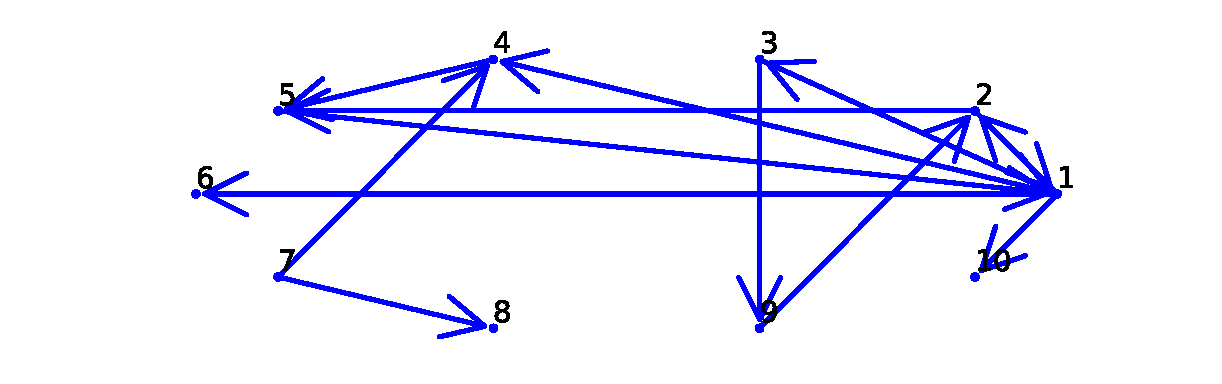
\includegraphics{or1.pdf} 
    \caption{Пример графа созданного с помощью данной модели}
    \label{orrnd_3}
\end{figure} 
На рисунке \ref{orrnd_3} приведена диаграмма графа созданного с помощью данной модели,
где $\alpha = 0.4,\beta = 0.4,\gamma =0.2, \delta_{\text{in}} = 2, \delta_{\text{out}} = 2$.
\subsection{Модель Бакли-Остхус}
Рассмотрим следущую \cite{buck} модификацию модели Боллобаша-Риодана. 
Дан граф с одной вершиной и петлей и параметр $a$. 
На  $i+1$-том шаге  вершина $i+1$ добавляется в граф, из нее 
проводится ребро в случайную вершину, которая выбирается со следушей вероятностью $P_{k,i+1} = \frac{\deg{k} + a }{(a+1)*(i+1) - 1}$,
$P_{i+1,i+1} = \frac{a}{(a+1)(i+1) - 1}$.

Рассмотрим реализацию данной модели.
\begin{figure}[H] 
\begin{lstlisting}[language=Python] 
    def add_edge(self):
        p = [(self.graph.deg(v) + self.a) / ((self.a+1) *
                                             (self.graph.k_vertecies() + 1) - 1) for v in self.graph.verticies()]
        p.append(self.a / ((self.a+1) * (self.graph.k_vertecies() + 1)-1))
        self.graph.add_vertex(self.nxt)
        v = choices(list(self.graph.verticies()), weights=p, k=1)[0]
        self.graph.add_edge(self.nxt, v)
        self.nxt += 1
\end{lstlisting}  
    \caption{Добавление вершины в граф}
    \label{os_1}
\end{figure} 
На риснуке \ref{os_1} представлен метод, реализующий добавление 
вершины в граф, согласно модели Бакли-Остхус.
\begin{figure}[H] 
    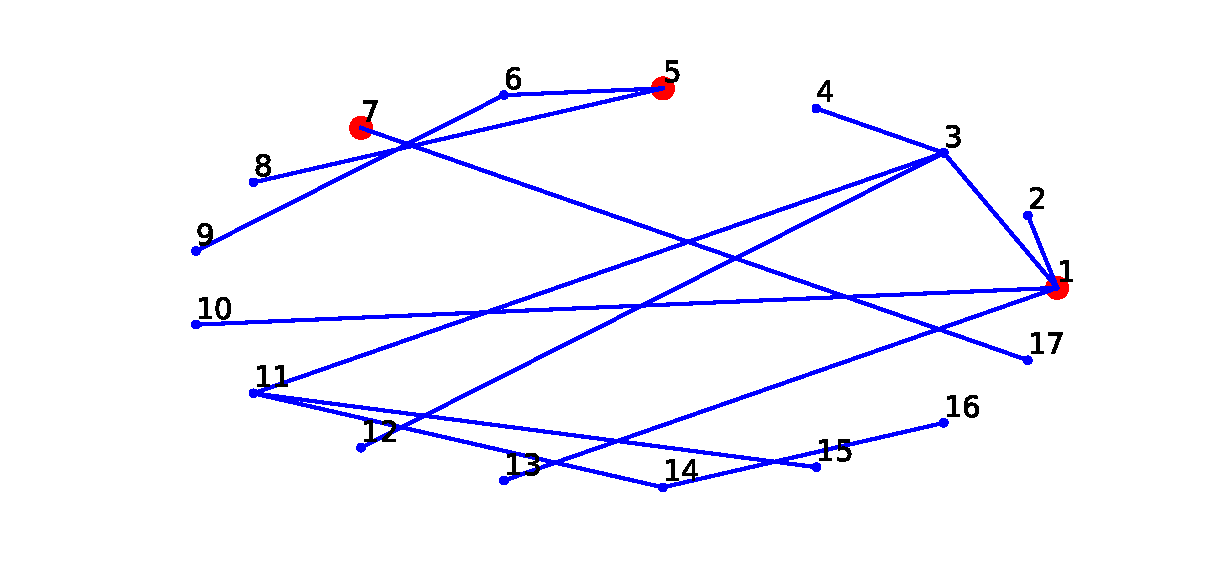
\includegraphics[scale=0.8]{os.pdf} 
    \caption{Пример графа, созданного с помощью модели Бакли-Остхус с параметром $a=2$}
    \label{os_2}
\end{figure} 
На рисунке \ref{os_2} представлен пример результата работы данной модели.
\subsection{Модель LCD}
Рассмотрим алгоритм генерации графа с помощью линейной хордовой
диаграммы (LCD):
\begin{enumerate}
    \item идем слева направо;
    \item добавляем в набор вершины, пока не встретим конец дуги;
    \item собранный набор становится вершиной графа, дуги становятся дугами графа;
\end{enumerate}
\begin{figure}[H] 
\begin{lstlisting}[language=Python] 
def __init__(self, n):
k = 2*n
    nums = list(range(1, k+1))
    self.left = []
    self.right = []
    for _ in range(n):
        l = choice(nums)
        nums.remove(l)
        r = choice(nums)
        nums.remove(r)
        self.left.append(l)
        self.right.append(r)
    v = []
    curr = []
    nums = list(range(1, k+1))
    for i in nums:
        curr.append(i)
        if i in self.right:
            v.append(curr.copy())
            curr = []
    g = Graph()
    for i, lst in enumerate(v, 1):
        g.add_vertex(i)
        for j, v2 in enumerate(lst):
            if v2 in self.left:
                r = self.right[j]
                for k in range(len(v)):
                    if r in v[k]:
                        g.add_edge(i, k+1)
    self.graph = g
\end{lstlisting}  
    \caption{Реализация LCD алгоритма.}
    \label{lcd1}
\end{figure} 
На рисунке \ref{lcd1} приведена реализация 
LCD алгоритма
\begin{figure}[H] 
    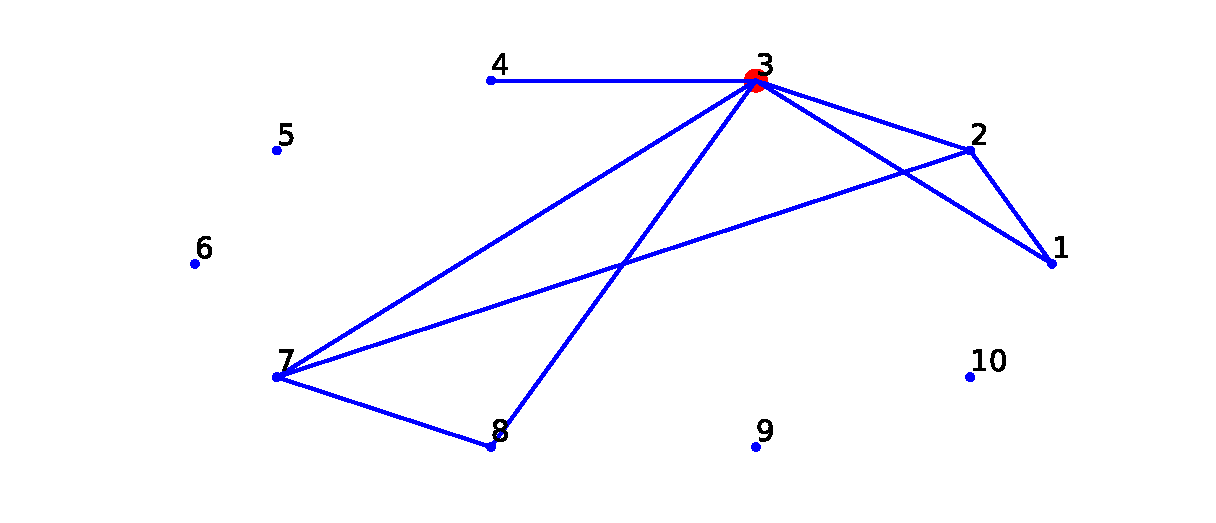
\includegraphics{lcd.pdf} 
    \caption{Граф, созданный с помощью LCD алгоритма}
    \label{lcd2}
\end{figure} 
На рисунке \ref{lcd2} приведен пример графа, созданного с помощью 
данного алгоритма.
\subsection{Модель копирования}
Пусть даны $\alpha \in (0,1)$ и 
 d-регулярный граф $d \ge  1$ , $V$ -- множество вершин этого графа. Рассмотрим алгоритм добавления вершины в граф:
 \begin{enumerate}
     \item выберем случайную вершину $p \in V$;
     \item добавляем d вершин по следущему правилу:
         с вероятностью $\alpha$ строим ребро из новой вершины 
         в  $p$ , c вероятностью $1 - \alpha$ строим
         ребро из новой вершины в  $i$-го соседа вершины  $p$;
 \end{enumerate}
 \begin{figure}[H] 
 \begin{lstlisting}[language=Python] 
    def add_vertex(self):
        v = self.j + 1
        self.j+=1
        p = choice(self.start_verticies)
        for i in range(self.d):
            if random() < self.alpha:
                self.graph.add_edge(p, v)
            else:
                self.graph.add_edge(list(self.graph.neib(p))[i], v)
 \end{lstlisting}  
     \caption{Метод, реализующий алгоритм добавления вершин,
     согласно модели копирования.}
     \label{cop1}
 \end{figure} 
 На рисунке \ref{cop1} приведен метод 
добавления вершин в граф, согласно модели копирования.
\begin{figure}[H] 
    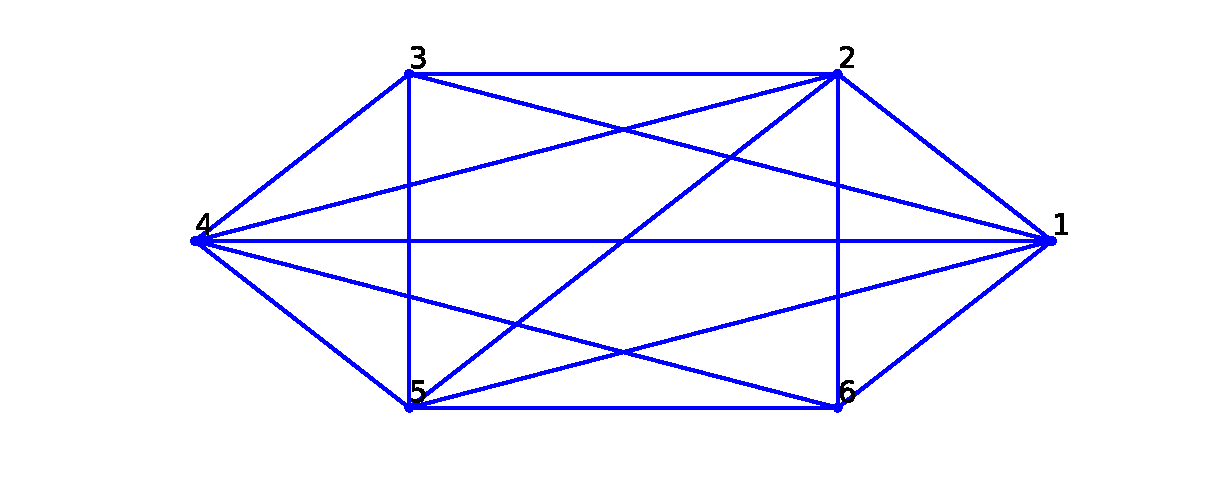
\includegraphics[scale=0.8]{cop1.pdf} 
    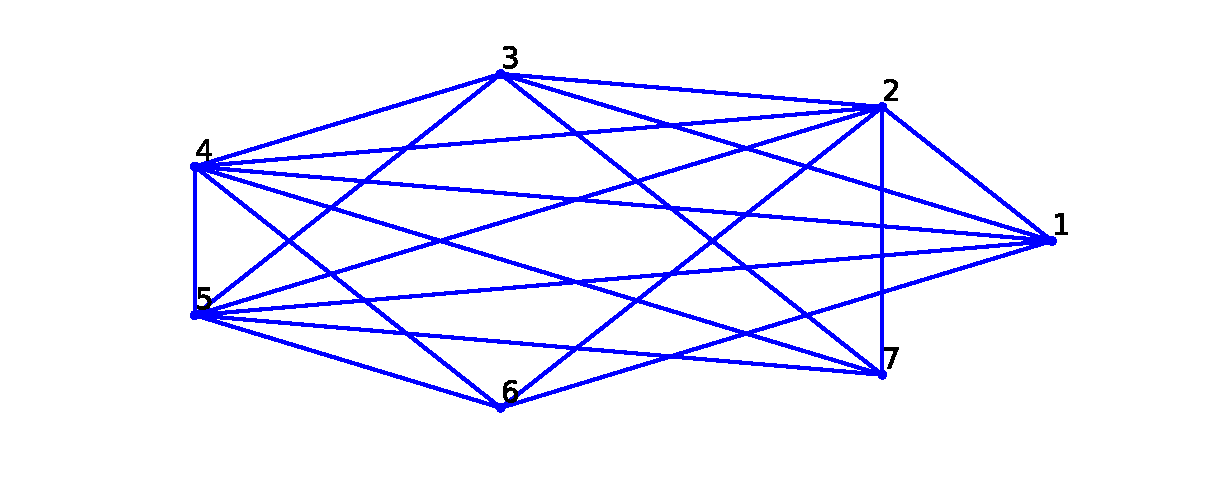
\includegraphics[scale=0.8]{cop2.pdf} 
    \caption{Результат добавления двух вершин в граф 
    с параметрами $d = 4,\alpha = 0.1$ согласно модели копирования.}
    \label{cop2}
\end{figure} 
На рисунке \ref{cop2} приведен пример генерации случайного графа согласно модели копирования.
\subsection{Модель Чунг-Ли}
Рассмотрим модель генерации случайного 
мультиграфа. Пусть нам дана степень каждой вершины,
степень $i$-ой вершины 
обозначим как  $d_{i}$. Граф генерируется следущим образом:
\begin{enumerate}
    \item строится множество $L$, которое состоит из
         $d_{i}$ копий вершины $i$;
    \item задаются случайные паросочетания на $L$;
    \item число парасочетаний между копиями  $u$ и  $v$ --
        число ребер между  $u$ и $v$;
\end{enumerate}
\begin{figure}[H] 
\begin{lstlisting}[language=Python] 
    def __init__(self, d: [int]):
        self.d = d
        self.l_set = []
        for i, elem in enumerate(d, 1):
            for _ in range(elem):
                self.l_set.append(i)

        self.edges = []
        for _ in range(sum(d)//2):
            a = choice(self.l_set)
            self.l_set.remove(a)
            b = choice(self.l_set)
            self.l_set.remove(b)
            self.edges.append((a, b))
        self.graph = MultiGraph()
\end{lstlisting}  
    \caption{Генерация случайного мультиграфа согласно модели ЧунгЛи.}
    \label{ch1}
\end{figure} 
На рисунке \ref{ch1} приведен код для создания случайного мультиграфа согласно данной модели.
\begin{figure}[H] 
    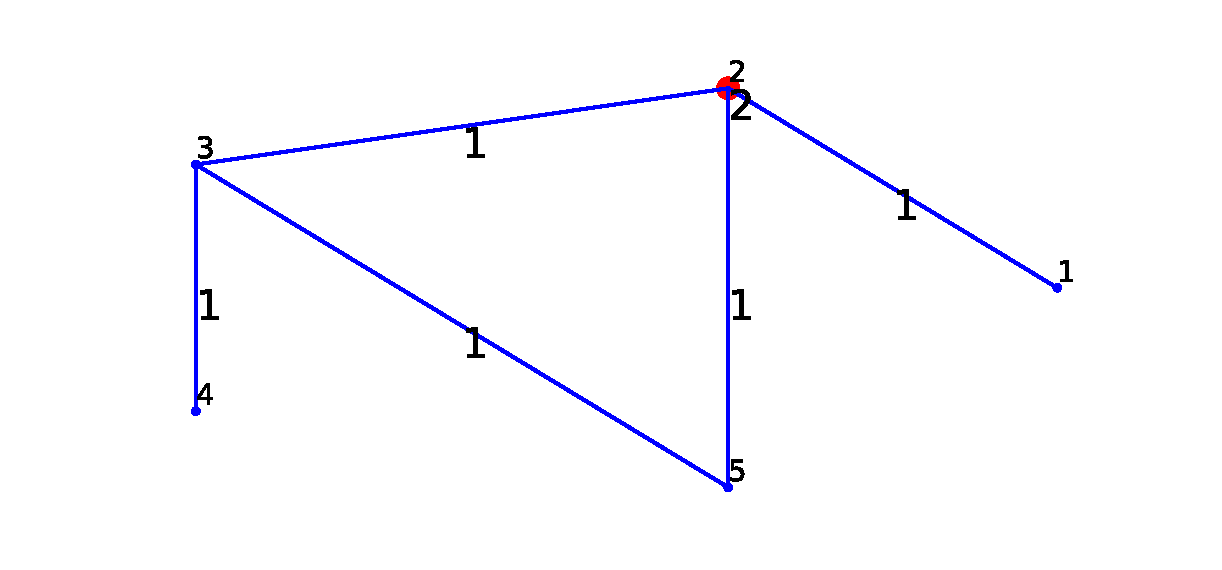
\includegraphics{ch.pdf}
    \caption{Мультиграф созданный с помощью модели Чунг-Ли,
    где $d = [1,5,2,1,2]$}
    \label{ch2}
\end{figure} 
Пример случайного мультиграфа, полученного согласно данно модели
приведен на рисунке \ref{ch2}.
\subsection{Модель Янсона-Лучака}
Рассмотрим набор вершин $v = \{v_1 \dots v_{n}\}$ и набор весов
$W = \{W_1 \dots W_{n}\}$.  Пусть
$\lambda_{ij} = \frac{W_{i} W_{j} }{n}$ -- математическое 
ожидание случайной величины $E_{ij}$, имеющей Пуассоновское распределение. Для вершин $i,j$ строится  $E_{ij}$ кратных ребер.
Получившийся мультиграф можно преобразовать в граф,
путем стягивания кратных ребер.
\begin{figure}[H] 
\begin{lstlisting}[language=Python] 
    def gen_graph(self):
        rng = np.random.default_rng()
        graph = MultiGraph()
        for (u, v) in combinations(range(1, len(self.weights)+1), 2):
            lamb = (self.weights[u-1]*self.weights[v-1]) / len(self.weights)
            for _ in range(int(lamb)):
                graph.add_edge(u,v)
            graph.add_vertecies((u,v))
        self.graph = graph
\end{lstlisting}  
    \caption{Генерация случайного графа согласно модели Янсона-Лучака.}
    \label{jason_1}
\end{figure} 
На рисунке \ref{jason_1} приведена реализация алгоритма 
создания случайного графа, согласно модели Янсона-Лучака.
Для генерации случайной величины используется библиотека <<numpy>> \cite{numpy}.
\begin{figure}[H] 
    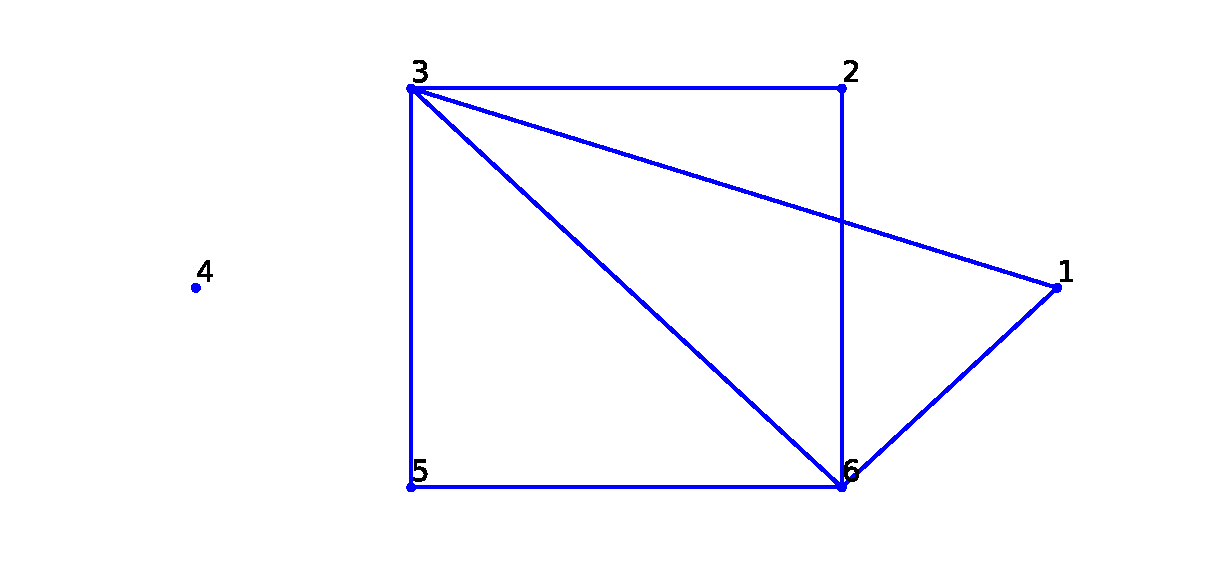
\includegraphics{jason.pdf} 
    \caption{Пример графа, созданного согласно модели Янсона-Лучака}
    \label{jason_2}
\end{figure} 
На рисунке \ref{jason_2} изображен граф, который был создан с 
помощью модели Янсона-Лучака, $w = \{2,2,3,1,3,2\} $.
\subsection{Генерация случайного геометрического графа}
Назовем граф $G(n,R)$ случайным геометрическим 
графом, если он получен путем размещения
на плоскости  $n$ вершин и две вершины
инцидентны, если евклидово расстояние между ними не превышает  $R$.
\subsubsection{Эффективный алгоритм генерации геометрических графов.}

 Пусть на 
плоскость наложена сетка, состоящая из 
квадратных ячеек с шагом  $\frac{R}{\sqrt{2} }$. Обозначим 
ячейку  $i$-тую по вертикали и  $j$-тую по вертикали как $L_{ij}$,
всего ячеек $L_{\text{size}}^2$. Назовем множество 
$\Omega_{ij} = \{(L_{kl} \mid  k \in -2 \dots 2, n \in -2 \dots 2 , 
0 \le  |k| + |m| < 3\}$ псевдоокрестностью $L_{ij}$
Рассмотрим следущий алгоритм генерации случайных
геометрических графов \cite{geo} :
\begin{enumerate}
    \item в каждой ячейке создается случайная вершина;
    \item для $i,j$ вершины создаются ребра смежные
        вершинам из  $\Omega_{ij}$, если расстояние между ними не превышает $R$;
    \item  $n_{\text{curr}} = n - L^2_{\text{size}}$ -- число несгенированных вершин;
    \item $N = n - L^2_{\text{size}}$ ;
    \item $p = \frac{1}{L^2_{\text{size}}}$ ;
    \item для $L_{ij}$ вычисляется $s_{ij} = \min(n_{\text{curr},B(N,p)})$, где $B(N,p)$ случайная величина распределенная по 
        биноминальному закону;
    \item в $L_{ij}$ создается $s_{ij}$ вершин;
    \item каждая созданная вершина соединяется с вершинами из
        $\Omega_{ij}$, если расстояние не превышает $R$;
    \item  $n_{\text{ curr }}$ уменьшается на $s_{ij}$ ;
    \item если $n_{\text{curr}} = 0$ то граф построен;
\end{enumerate}
Данный алгоритм является достаточно эффективным и
создает графы похожие на реальные структуры, такие 
как беспроводные сети.
\subsubsection{Реализация алгоритма генерации геометрических графов}
Геометрический граф будет реализован с 
помощью класса <<GeoGraph>>, который 
является потомком класса <<Graph>>. Для
реализации веришн был реализован класс <<Node>>, имеющий следущие
поля и методы:
\begin{enumerate}
    \item поле <<x>> -- координата по оси  $X$;
    \item  поле  <<y>> -- координата по оси $Y$;
    \item метод  <<dist>> -- вычисляет евклидово расстояние между 
        двумя вершинами;
\end{enumerate}
Рассмотрим реализацию на языке программирования Python.

\begin{figure}[H] 
\begin{lstlisting}[language=Python] 
@dataclass(frozen=True)
class Node:
    x: float
    y: float
\end{lstlisting}  
    \caption{Определение класса <<Node>>}
    \label{pynode_1}
\end{figure} 
\begin{figure}[H] 
\begin{lstlisting}[language=Python] 
    def dist(self, other):
        return sqrt((self.x - other.x) ** 2 + (self.y - other.y)**2)
\end{lstlisting}  
    \caption{Метод для вычисления еклидового расстояния между двумя вершинами.}
    \label{pynode_2}
\end{figure} 
На рисунках \ref{pynode_1}, \ref{pynode_2} приведена реализация вершины 
геометричесого графа.

Модель генерации случайного геометрического графа была 
определена в классе <<GeoGraphRndModel>>. В данном 
классе был определен метод инициализации и метод создания графа.
\begin{figure}[H] 
\begin{lstlisting}[language=Python] 
    def __init__(self, r, n):
        self.n = n
        self.r = r
        self.l_step = r/(sqrt(2))
        self.l_size = int(sqrt(n))
        self.grid = Grid(self.l_size)
        self.gen_graph()
\end{lstlisting}  
    \caption{Инициалиация модели генерации случайного геометрического графа.}
    \label{geornd1}
\end{figure} 
На рисунке \ref{geornd1} приведен метод создания 
модели случайного геометрического графа. Рассмотрим
реализацию алгоритма генерации случайного графа.
\begin{figure}[H] 
\begin{lstlisting}[language=Python] 
    def gen_graph(self):
        self.graph = GeoGraph()
        for lst in self.grid.grid.values():
            self.graph.add_vertecies(lst)
        for i in range(self.l_size):
            for j in range(self.l_size):
                for n1 in self.grid.grid[i, j]:
                    omega = self.grid.omega(i, j)
                    for n2 in omega:
                        if n1.dist(n2) <= self.r and n2 != n1:
                            self.graph.add_edge(n1, n2)
        N = self.n - self.l_size**2
        p = (1/self.l_size)**2
        n_curr = self.n - self.l_size**2
        for i in range(self.l_size):
            for j in range(self.l_size):
                s = binomial(N, p)
                s = min(s, n_curr)
                for _ in range(s):
                    n = Node(i+random(), j+random())
                    for n2 in self.grid.grid[i, j]:
                        self.graph.add_edge(n, n2)
                    omega = self.grid.omega(i, j)
                    for n2 in omega:
                        if n.dist(n2) <= self.r:
                            self.graph.add_edge(n, n2)
                    self.grid.grid[i, j].append(n)
                    self.graph.add_vertex(n)
                n_curr -= s
                if n_curr <= 0:
                    break
\end{lstlisting}  
    \caption{Реализация алгоритма генерации случайного геометрического
    графа}
    \label{geornd2}
\end{figure} 
На рисунке \ref{geornd2} приведен метод, 
реализующий генерацию случайного геометрического графа.

Рассмотрим примеры графов, созданных с помощью данного алгоритма.
\begin{figure}[H] 
    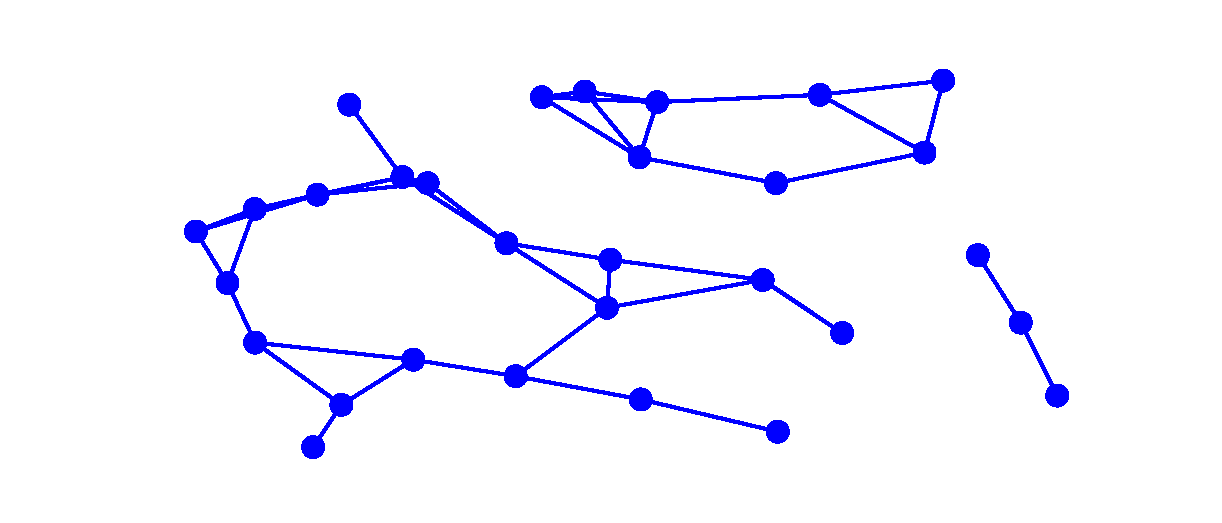
\includegraphics{geo301.pdf} 
    \caption{Случайный геометрический граф, $n=30$,  $R=1$}
    \label{geoex_1}
\end{figure} 
\begin{figure}[H] 
    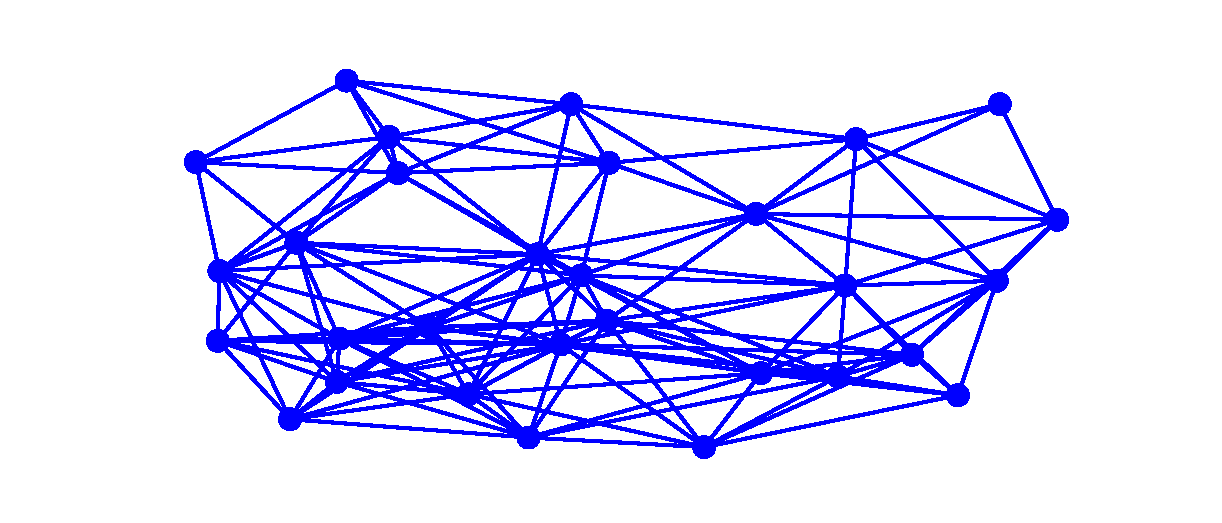
\includegraphics{geo302.pdf} 
    \caption{Случанйый геометрический граф, $n=30$,  $R=2$}
    \label{geoex_2}
\end{figure} 
На рисунках \ref{geoex_1},\ref{geoex_2} приведены 
примеры графов, созданных c помощью алгоритма генерации
случайных геометрических графов.
